\chapter{Estudio de tecnologías y decisiones de diseño}
\label{ch:estudio-tecnologias}

Este capítulo describe las tecnologías que componen Parky y justifica cada elección frente a las alternativas consideradas. Para cada herramienta se explica qué función cumple en el sistema, por qué se prefirió sobre las alternativas consideradas y qué compromisos implica la elección.

% ============================================================
\section{Lenguajes de programación y frameworks}
\label{sec:lenguajes}

La arquitectura separa con claridad dos ámbitos: el \textit{frontend}, ejecutado en el navegador o en el dispositivo Android, y el \textit{backend}, delegado íntegramente a servicios externos gestionados. Esta separación permitió concentrar el desarrollo en la lógica de negocio y la experiencia de usuario sin gestionar servidores propios.

% ------------------------------------------------------------
\subsection{Frontend}
\label{subsec:frontend}

El frontend de Parky se organiza en tres capas funcionales: el lenguaje y el sistema de tipos, el framework de renderizado con su cadena de herramientas, y la capa de gestión de datos, formularios y estilos.

\paragraph{Lenguaje y tipado.}
Todo el código fuente está escrito en \textit{TypeScript 5}~\cite{typescript2024} porque su compilador actúa como primera línea de defensa: detecta incompatibilidades de tipo, propiedades inexistentes y posibles valores nulos antes de que el código llegue al navegador. Esta garantía es especialmente valiosa en Parky, donde los errores de tipo tienen consecuencias directas sobre la integridad del negocio. Por ejemplo, una validación incorrecta en el intervalo de reserva puede crear solapamientos, y un error en el desglose de precio base, comisión e IGIC puede generar cargos incorrectos en Stripe. Los componentes de React se expresan en \textit{JSX}\footnote{\textbf{JSX} (\textit{JavaScript XML}): Extensión de sintaxis que permite escribir marcado similar a HTML dentro del código JavaScript.}, y \textit{SWC}\footnote{\textbf{SWC} (\textit{Speedy Web Compiler}): Transpilador escrito en Rust que reemplaza a Babel. Es entre 20 y 70 veces más rápido en compilaciones en frío.} se encarga de transformar ese código a JavaScript puro antes de enviarlo al navegador.

\paragraph{Framework y renderizado.}
La interfaz se construye con \textit{React 18.3.1}~\cite{react2024}. El argumento determinante para elegir esta versión fue el \textit{modo concurrente}: características como \texttt{useTransition} y \texttt{startTransition} permiten marcar como no urgentes las actualizaciones costosas en componentes React —por ejemplo, refrescar el listado de plazas disponibles al mover el mapa— de modo que el motor puede aplazar esa actualización para atender primero los gestos táctiles del usuario, evitando que los paneles de filtros o resultados bloqueen la interacción durante cargas intensivas.

El empaquetador es Vite 6.4.1~\cite{vitejs2024}, que acelera el ciclo de desarrollo al evitar recompilar toda la aplicación ante cada cambio, y optimiza el código para  producción eliminando automáticamente las partes no utilizadas. El enrutado usa \textit{React Router DOM 7}~\cite{reactrouter2024}, configurado con \textit{lazy loading} para cargar el código de cada pantalla únicamente cuando el usuario la visita, lo que reduce el tiempo de carga inicial de la aplicación.

El factor que descartó las alternativas fue la integración con \textit{Capacitor}, el adaptador que empaqueta la aplicación web como APK nativo de Android. Angular quedó descartado por su curva de aprendizaje y menor afinidad con Capacitor; Vue y Svelte ofrecen mejoras de rendimiento notables pero su ecosistema para integraciones híbridas móviles es mucho más reducido. La \autoref{tab:frameworks-comparativa} resume los criterios decisivos:

\begin{table}[htbp]
  \centering
  \caption{Comparativa de frameworks JavaScript de frontend para el desarrollo de Parky.}
  \label{tab:frameworks-comparativa}
  \begin{tabularx}{\textwidth}{lXXXX}
    \toprule
    \textbf{Criterio}        & \textbf{React 18} & \textbf{Vue 3} & \textbf{Angular 17} & \textbf{Svelte 4} \\
    \midrule
    Modo concurrente         & Sí (v18)          & No             & No                  & No                \\
    App nativa (Capacitor)   & Completa          & Limitada       & Limitada            & Experimental      \\
    Ecosistema híbrido móvil & Muy amplio        & Reducido       & Reducido            & Muy reducido      \\
    \bottomrule
  \end{tabularx}
\end{table}

\paragraph{Estado, formularios y estilos.}
La sincronización de datos con el servidor se gestiona con \textit{TanStack Query v5}~\cite{tanstack_query2024}\footnote{\textbf{TanStack Query}: biblioteca de gestión de estado asíncrono que abstrae la caché, el ciclo de vida y la sincronización de datos remotos en aplicaciones React.}, que mantiene la interfaz actualizada automáticamente sin que el desarrollador gestione manualmente cuándo y cómo refrescar los datos. Esto es especialmente relevante en Parky, donde la disponibilidad de una plaza puede cambiar en cualquier momento por una reserva concurrente.

Los formularios (alta de plaza, inicio de sesión, selección de intervalo de reserva) se gestionan con \textit{React Hook Form 7}\footnote{\textbf{React Hook Form}: biblioteca de gestión de formularios que registra los campos mediante refs en lugar de estado de React, minimizando los re-renders durante la edición.}. A diferencia del enfoque estándar de React, los campos no provocan un re-render de la interfaz en cada pulsación de teclado, lo que importa especialmente en formularios con validaciones cruzadas como el selector de intervalo horario de una reserva.

El sistema de estilos usa \textit{Tailwind CSS 4.1.3}~\cite{tailwindcss2024} \footnote{\textbf{Tailwind CSS}: framework de estilos utility-first que compone el diseño visual mediante clases atómicas aplicadas directamente en el marcado, en lugar de hojas CSS por componente.}. Los componentes de interfaz se construyen sobre Radix UI\footnote{\textbf{Radix UI}: biblioteca de componentes primitivos para React que garantiza accesibilidad por defecto sin imponer estilos propios.}, que garantiza un comportamiento accesible por defecto (gestión de foco, navegación por teclado, atributos ARIA, etc.) de modo que Tailwind controla completamente la apariencia visual sin fricciones.

% ------------------------------------------------------------
\subsection{APIs externas de cartografía y geocodificación}
\label{subsec:apis-cartografia}

En Parky la localización geográfica no es un complemento sino el núcleo de la experiencia: el arrendatario busca plazas dentro del área visible del mapa, las visualiza como marcadores geoposicionados y accede a la dirección exacta del garaje. Esto exige dos capacidades independientes: renderizar mapas interactivos y convertir direcciones de texto en coordenadas geográficas.

\paragraph{Leaflet.}
La visualización cartográfica usa \textit{Leaflet 1.9.4}~\cite{leafletjs2024} con el adaptador React-Leaflet 4.2.1. La alternativa natural era la API de \textit{Google Maps}, descartada por su modelo de facturación por volumen. Leaflet es \textit{open source} (bajo licencia BSD-2), sin coste por carga de mapa, y su rendimiento en dispositivos Android de gama media es suficiente para los casos de uso de Parky.

\paragraph{OpenCage Geocoding API.}
La conversión entre direcciones de texto y coordenadas geográficas usa \textit{OpenCage Geocoding API}~\cite{opencage2024}. Este servicio agrega datos de OpenStreetMap, Geonames y otras fuentes abiertas con soporte para direcciones canarias, lo que es fundamental para la aplicación. El plan gratuito incluye 2.500 peticiones diarias, suficiente para el volumen esperado durante la fase de prototipado.

% ------------------------------------------------------------
\subsection{Backend}
\label{subsec:backend}

Se evaluó desarrollar un servidor a medida con \textit{Node.js} o \textit{Python} frente al uso de plataformas \textit{BaaS}\footnote{\textbf{BaaS (Backend-as-a-Service):} Modelo donde un proveedor externo aloja la infraestructura central del servidor —almacenamiento, autenticación, base de datos— y el desarrollador la consume a través de APIs documentadas.}, pero se optó por \textit{Supabase}~\cite{supabase2024} por tres razones.

Supabase cuenta con una capa de autenticación que gestiona el cifrado de contraseñas, los flujos OAuth (Google) de forma nativa y las sesiones mediante \textit{JWT}\footnote{\textbf{JWT} (\textit{JSON Web Token}): estándar RFC 7519 que define un formato compacto para transmitir información entre partes como objeto JSON firmado criptográficamente.}, eliminando la necesidad de implementar y auditar un sistema de identidades propio. También cuenta con un almacenamiento de objetos que gestiona las imágenes de garajes y perfiles con políticas de acceso integradas que impiden que un usuario modifique recursos ajenos. Por último y más importante, para los pagos, la plataforma cuenta con integración con \textit{Stripe Connect}\footnote{\textbf{Stripe Connect}: arquitectura de pagos de Stripe para \textit{marketplaces} que separa y liquida automáticamente los fondos entre las partes.} por medio de Edge Functions, que calculan la comisión de la plataforma, el \textit{IGIC} y transfieren el saldo neto directamente a la cuenta bancaria del propietario del garaje sin que los fondos pasen por una cuenta bancaria central, lo que simplifica la fiscalidad.

Un desarrollo backend propio habría requerido implementar estos tres sistemas desde cero, con la carga de mantenimiento y la superficie de ataque que eso implica en un equipo de una sola persona.

% ------------------------------------------------------------
\subsection{Base de datos}
\label{subsec:bbdd}

Se compararon el modelo relacional y el modelo documental para la capa de persistencia. El dominio de Parky es inherentemente relacional: una reserva vincula a un usuario con una plaza, que pertenece a un garaje, durante un intervalo de tiempo con un pago asociado. \textit{MongoDB}~\cite{mongodb2024} exigiría replicar esa cadena en múltiples documentos, con el riesgo de inconsistencia ante una operación fallida a mitad de ejecución. Es por eso que se eligió \textit{PostgreSQL}~\cite{postgresql2024} porque resuelve esa inconsistencia con integridad referencial mediante \textit{foreign keys}\footnote{\textbf{Foreign key} (clave foránea): columna que referencia la clave primaria de otra tabla, garantizando que no puedan existir reservas de plazas inexistentes o registros huérfanos.} y \textit{transacciones ACID}\footnote{\textbf{ACID}: propiedades de Atomicidad, Consistencia, Aislamiento y Durabilidad que garantizan que las operaciones de base de datos se ejecutan completamente o no se ejecutan en absoluto.}.

Dentro de \textit{PostgreSQL 15} se usan dos características avanzadas: las \textit{políticas RLS} que garantizan que cada usuario solo pueda leer sus propias reservas y los \textit{triggers PL/pgSQL} que comprueban, antes de confirmar cualquier reserva, que no exista solapamiento horario en la misma plaza, manteniendo la consistencia incluso ante peticiones simultáneas.

% ============================================================
\section{Entorno de desarrollo}
\label{sec:entorno}

\paragraph{Editor de código.}
El entorno de desarrollo es \textit{Visual Studio Code}~\cite{vscode2026}. Frente a IDEs\footnote{\textbf{IDE} (\textit{Integrated Development Environment}): entorno que agrupa editor, compilador y depurador en una única aplicación.} basados en IntelliJ, su consumo de memoria es sensiblemente menor, lo que resulta determinante en el desarrollo híbrido con Capacitor, donde el emulador de Android debe estar abierto en paralelo. Además, integra de forma nativa el servidor de TypeScript, por lo que el análisis de tipos en el editor es idéntico al de la compilación real.

\paragraph{Control de versiones.}
El control de versiones usa \textit{Git}~\cite{git2024} con \textit{GitHub}~\cite{github2024} como repositorio remoto. Esta combinación no solo documenta el historial de cambios por fases de desarrollo, sino que actúa como punto de integración con el pipeline de despliegue continuo de Vercel: cada commit en la rama principal desencadena automáticamente un nuevo despliegue en producción.

\paragraph{Diseño de interfaces.}
El diseño visual previo a la implementación se realizó con \textit{Figma}~\cite{figma2024}, que permitió validar la disposición de pantallas, la paleta de colores y las distancias entre elementos antes de traducirlos a clases de Tailwind CSS. Trabajar con un prototipo de alta fidelidad redujo el número de decisiones de diseño durante el desarrollo, concentrando ese esfuerzo en una fase anterior donde el coste de cambio es menor. La figura~\ref{fig:figma-vs-produccion-home} muestra la evolución entre el prototipo inicial y la pantalla principal en producción.

\begin{figure}[H]
  \centering
  \begin{minipage}{0.48\textwidth}
    \centering
    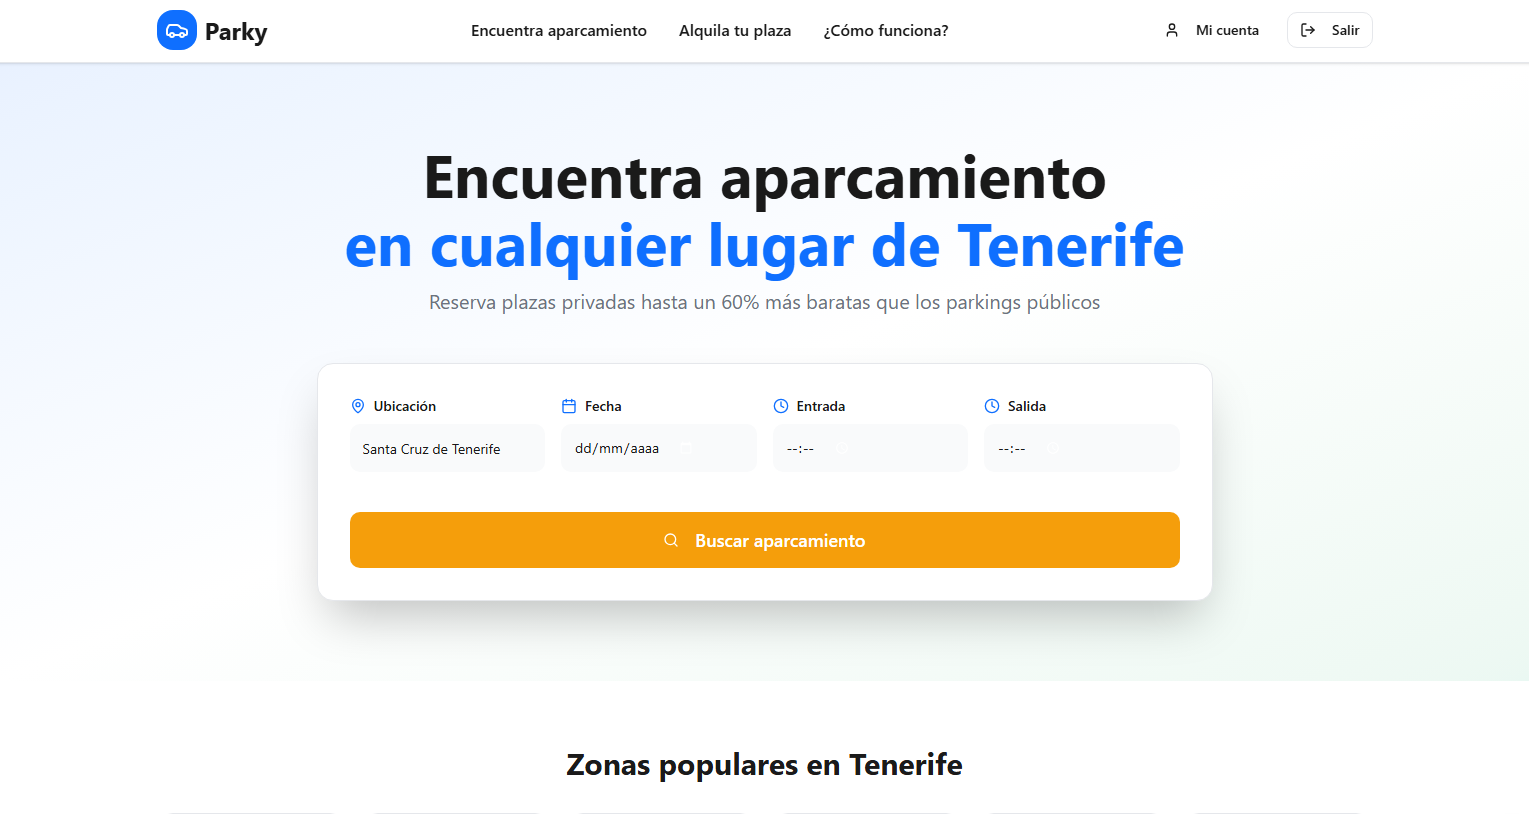
\includegraphics[width=\textwidth]{images/assets/FIGMA_HOME}
  \end{minipage}%
  \hfill
  \begin{minipage}{0.48\textwidth}
    \centering
    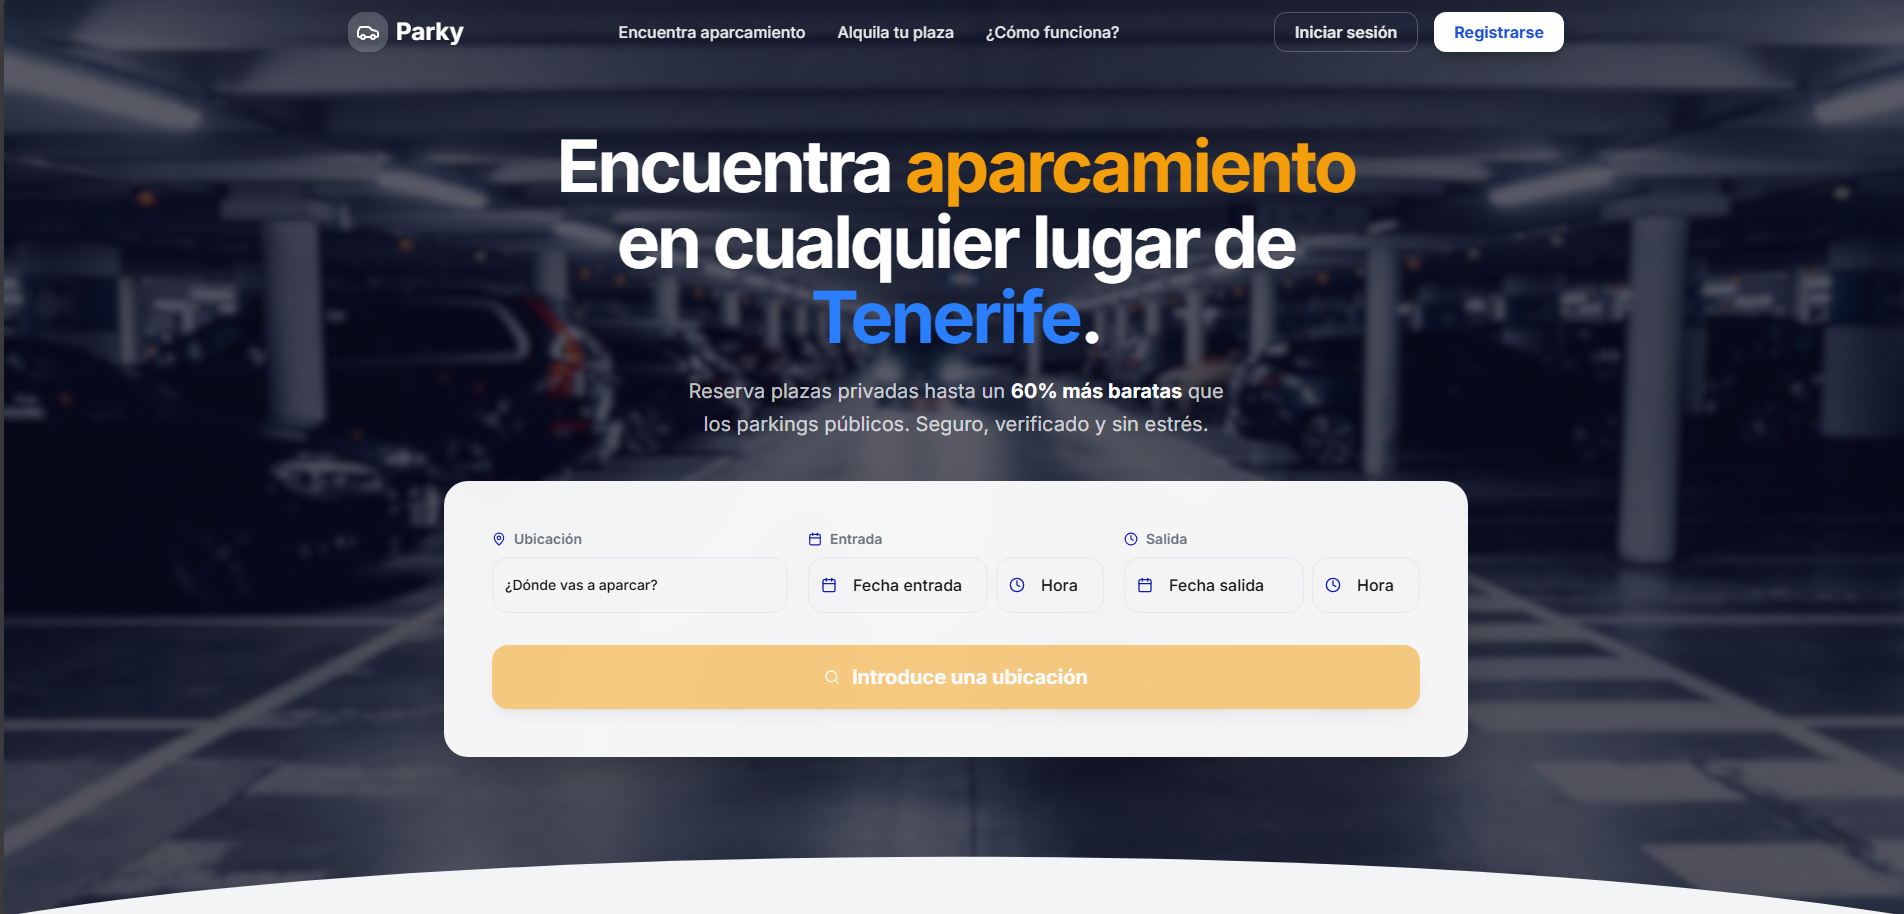
\includegraphics[width=\textwidth]{images/assets/PARKY_HOME}
  \end{minipage}
  \caption{Comparativa entre el prototipo en Figma (izquierda) y la pantalla principal de Parky en producción (derecha).}
  \label{fig:figma-vs-produccion-home}
\end{figure}

% ============================================================
\section{Plataformas de despliegue}
\label{sec:despliegue}

\paragraph{Web: Vercel.}
La versión web se despliega en \textit{Vercel}~\cite{vercel2024}, elegido por su integración nativa con GitHub ya que cada commit en la rama principal desencadena automáticamente una nueva compilación y distribución en su CDN global, sin configuración adicional. Gestiona además los certificados TLS de forma automática. El dominio público de la página se registró en One.com~\cite{onecom2024} y se enlazó a Vercel mediante registros DNS.

\paragraph{Android: Capacitor.}
La aplicación Android se genera con \textit{Capacitor 8.1.0}~\cite{capacitor2024}, que encapsula la aplicación web dentro de una WebView nativa. A diferencia de React Native, que requiere reescribir los componentes en primitivas nativas, Capacitor reutiliza las vistas TypeScript/HTML sin modificaciones, lo que permite mantener una única base de código para web y Android. El APK final se compila desde Android Studio sin modificar ningún componente de React.

% ============================================================
\section{Análisis de alternativas y decisiones de diseño}
\label{sec:dificultades}

La tabla~\ref{tab:baas-comparativa} recoge la comparativa de plataformas BaaS que determinó la elección de Supabase como infraestructura central del proyecto.

\begin{table}[htbp]
  \centering
  \caption{Comparativa de plataformas BaaS frente a las necesidades de Parky.}
  \label{tab:baas-comparativa}
  \begin{tabularx}{\textwidth}{lXXX}
    \toprule
    \textbf{Característica} & \textbf{Supabase}~\cite{supabase2024}
                            & \textbf{Firebase}~\cite{firebase2024}
                            & \textbf{AWS Amplify}~\cite{awsamplify2024} \\
    \midrule
    Motor de base de datos  & PostgreSQL (relacional)
                            & Firestore (documental)
                            & DynamoDB / Aurora Serverless               \\
    Consultas relacionales  & SQL nativo con JOINs
                            & Limitadas, sin JOINs
                            & Posibles con Aurora Serverless             \\
    Row Level Security      & Nativo en PostgreSQL
                            & No disponible
                            & No disponible                              \\
    Autenticación           & Nativo (email, OAuth, MFA)
                            & Authentication integrado
                            & Amazon Cognito                             \\
    Triggers y funciones    & PL/pgSQL + Edge Functions (Deno)
                            & Cloud Functions (externo)
                            & Lambda (externo)                           \\
    Modelo de datos         & Normalizado, tipado
                            & Flexible, sin esquema
                            & Mixto (NoSQL o relacional)                 \\
    Límite tier gratuito    & 500 MB / 2 proyectos
                            & 1 GB (Spark Plan)
                            & 12 meses AWS Free Tier                     \\
    \bottomrule
  \end{tabularx}
\end{table}

Tanto Firebase como AWS Amplify están pensados para modelos de datos documentales y escalan bien en ese contexto, pero el dominio de Parky no encaja ahí. La cadena reserva\,---\,usuario\,---\,plaza\,---\,garaje\,---\,intervalo\,---\,pago se expresa de forma natural en tablas relacionadas mediante JOINs; trasladarla a Firestore obligaría a replicar datos en varios documentos, lo que introduce riesgo de inconsistencia ante cualquier escritura parcial fallida. AWS Amplify ofrece Aurora Serverless como salida relacional, pero su configuración es considerablemente más compleja y carece de RLS nativo, lo que habría obligado a gestionar el aislamiento de datos entre roles desde la capa de aplicación en lugar de resolverlo directamente en el esquema de base de datos.

El principal compromiso de Supabase es su plan gratuito: 500~MB de almacenamiento y pausa automática del proyecto tras 7 días de inactividad. Para un prototipo universitario ambos límites son asumibles, pero una versión comercial requeriría migrar al plan Pro (\$25/mes).